\documentclass[xcolor=dvipsnames,aspectratio=169]{beamer}
\usepackage[utf8]{inputenc}
\usetheme{Warsaw}
\usepackage{pgfpages}

% -----------------------------------------------------------------------------
% Notes toggle
% Compile with \def\NOTES{} before \input if you want notes-only output.
% -----------------------------------------------------------------------------
\newif\ifnotes
\ifdefined\NOTES\notestrue\fi
\ifnotes
  \setbeameroption{show only notes}
\else
  \setbeameroption{hide notes}
\fi

% -----------------------------------------------------------------------------
% Shared formatting
% -----------------------------------------------------------------------------
\setcounter{tocdepth}{2}

% =============================================================================
% Theme settings
% =============================================================================

% --- Core theme colors ---
\definecolor{ThemePrimary}{rgb}{0.0745, 0.1608, 0.2941}   % deep blue
\definecolor{ThemeSecondary}{rgb}{0.8667, 0.2039, 0.0118} % warm red/orange
\definecolor{ThemeAccent}{rgb}{0.1137, 0.3451, 0.6549}    % medium blue
\definecolor{ThemeLight}{rgb}{0.9725, 0.9804, 0.9882}     % near white
\definecolor{ThemeText}{rgb}{0.10, 0.10, 0.10}

% --- Optional extra palette ---
\definecolor{ThemeHighlight}{rgb}{0.9608, 0.5294, 0.1176}
\definecolor{ThemeSoftBlue}{rgb}{0.0000, 0.6235, 0.8314}
\definecolor{ThemeSoftNavy}{rgb}{0.1176, 0.2196, 0.4667}

% =============================================================================
% Beamer color settings
% =============================================================================

\setbeamercolor{palette primary}{bg=ThemePrimary,fg=ThemeLight}
\setbeamercolor{structure}{fg=ThemePrimary}
\setbeamercolor{section in toc}{fg=ThemePrimary}
\setbeamercolor{frametitle}{bg=ThemeSecondary,fg=ThemeLight}
\setbeamercolor{frametitle right}{bg=ThemePrimary}
\setbeamercolor{titlelike}{bg=ThemeSecondary,fg=ThemeLight}

% Optional tweaks you can enable later if desired:
% \setbeamercolor{block title}{bg=ThemePrimary,fg=ThemeLight}
% \setbeamercolor{block body}{bg=ThemeLight,fg=ThemeText}
% \setbeamercolor{section in head/foot}{bg=ThemeSoftNavy,fg=ThemeLight}
% \setbeamercolor{subsection in head/foot}{bg=ThemePrimary,fg=ThemeLight}

% =============================================================================
% Footline with page numbers
% =============================================================================

\defbeamertemplate*{footline}{shadow theme}{
    \leavevmode
    \hbox{%
        \begin{beamercolorbox}[
            wd=.5\paperwidth,
            ht=2.5ex,
            dp=1.125ex,
            leftskip=.3cm plus1fil,
            rightskip=.3cm
        ]{author in head/foot}
            \usebeamerfont{author in head/foot}\hfill\insertshortauthor
        \end{beamercolorbox}%
        \hskip0pt%
        \begin{beamercolorbox}[
            wd=.5\paperwidth,
            ht=2.5ex,
            dp=1.125ex,
            leftskip=.3cm,
            rightskip=.3cm plus1fil
        ]{title in head/foot}
            \usebeamerfont{title in head/foot}%
            \insertshorttitle\hfill\insertframenumber\,/\,\inserttotalframenumber
        \end{beamercolorbox}%
    }
    \vskip0pt
}

% =============================================================================
% Headline with current section / subsection
% =============================================================================

\setbeamertemplate{headline}{%
  \leavevmode
  \hbox{%
    \begin{beamercolorbox}[
        wd=.5\paperwidth,
        ht=2.1ex,
        dp=0.7ex,
        leftskip=0.3cm
    ]{section in head/foot}
      \usebeamerfont{section in head/foot}\insertsectionhead
    \end{beamercolorbox}%
    \begin{beamercolorbox}[
        wd=.5\paperwidth,
        ht=2.1ex,
        dp=0.7ex,
        rightskip=0.3cm
    ]{subsection in head/foot}
      \usebeamerfont{subsection in head/foot}\hfill\insertsubsectionhead
    \end{beamercolorbox}%
  }%
}

% =============================================================================
% Automatic outline slides
% =============================================================================

\AtBeginSection[]{
    \begin{frame}{Outline}
        \tableofcontents[currentsection]
    \end{frame}
}

\AtBeginSubsection[]{
    \begin{frame}{Outline}
        \tableofcontents[currentsection,currentsubsection]
    \end{frame}
}

% =============================================================================
% Figure / table packages
% =============================================================================

\usepackage{graphicx}   % figures
\usepackage{float}      % figure/table placement
\usepackage{rotating}   % rotated figures/tables
\usepackage{caption}    % captions
\usepackage{subcaption} % subfigures
\usepackage{makecell}   % table formatting
\usepackage{longtable}  % multipage tables
\usepackage{array}      % custom columns
\usepackage{tabularx}   % flexible-width tables
\usepackage{booktabs}   % professional tables

\newcolumntype{L}{>{\raggedright\arraybackslash}m{4cm}}
\newcolumntype{R}[1]{>{\raggedright\arraybackslash\hspace{0pt}\vspace{-0.25cm}}p{#1}}

% =============================================================================
% Math packages
% =============================================================================

\usepackage{amsfonts}
\usepackage{mathrsfs}
\usepackage{amsmath}
\usepackage{amssymb}
\usepackage{amsthm}
\usepackage{mathtools}
\usepackage{steinmetz}

% =============================================================================
% Chemistry / units
% =============================================================================

\usepackage[version=4]{mhchem}
\usepackage{chemformula}

\usepackage{siunitx}
\sisetup{locale = DE}
\sisetup{output-decimal-marker = {.}}

% =============================================================================
% Code / URL / verbatim
% =============================================================================

\usepackage{listings}
\usepackage{url}
\usepackage{verbatim}

% =============================================================================
% Helper
% =============================================================================



% =============================================================================
% End of format file
% =============================================================================

% Diagrams (talk-specific)
\usepackage{tikz}
\usetikzlibrary{arrows.meta,positioning,fit,calc}

% -----------------------------------------------------------------------------
% Presentation metadata
% -----------------------------------------------------------------------------
\newcommand{\TalkTitle}{Ha \& Schmidhuber (2018) - World Models}
\newcommand{\TalkAuthor}{Soo Min Kimm}
\newcommand{\TalkInstitute}{}
\newcommand{\TalkDate}{08/10/26}

\title{\TalkTitle}
\subtitle{Literature Review}
\author{\TalkAuthor}
\institute{\TalkInstitute}
\date{\TalkDate}


% Figure captions and sources stay directly below their figures.
\newcommand{\figsource}[2]{%
    \par\smallskip{\scriptsize\color{ThemeText}%
    #1\par
    \href{https://arxiv.org/abs/1803.10122}{Source: Ha \& Schmidhuber (2018)}, #2\par}%
}



% Automatic section outlines.
\AtBeginSection[]{
    \begin{frame}{Outline}
        \tableofcontents[currentsection,subsectionstyle=show/show/hide]
    \end{frame}
}

% Keep subsection navigation without adding a separate outline for each slide.
\AtBeginSubsection[]{}

\begin{document}

\begin{frame}
    \titlepage
    \note{
        The paper asks how a learned internal model can help an agent act.
        We will examine two uses: predictive features for a controller, and a learned simulator for training it.
        The main design separates vision, prediction, and control, so reward optimisation can focus on a small controller.
        Here is the route through those ideas.
    }
\end{frame}

\begin{frame}{Outline}
    \tableofcontents[hideallsubsections]
    \note{
        We start with the world, the agent, and their interaction loop.
        Then we define a world model and examine V, M, and C.
        The two experiments show how this architecture supports control in the actual game and training inside a dream.
        We finish by comparing its design with recent models.
        First, which part chooses actions, and which part responds?
    }
\end{frame}

\section{World, Agent, and World Model}
\begin{frame}{World and Agent}
    \begin{block}{World}
        The system whose changes matter for the task: its entities, their current state,
        and how they evolve under actions. In robotics, this includes the robot's body
        and its surroundings.
    \end{block}

    \begin{block}{Agent}
        The decision-making system that receives observations and chooses actions
        to pursue a goal. Its rule for choosing actions is called a \textbf{policy}.
    \end{block}
    \note{
        The world is the task-relevant system we want to understand and influence.
        For a robot pushing a cup, it includes the cup, table, and robot's physical body.
        The agent makes decisions; its policy selects actions from the information available.
        An agent can also contain perception, memory, and prediction.
        Here the controller chooses commands, while the robot's body and surroundings respond.
        Let us follow one interaction between them.
    }
\end{frame}

\begin{frame}{The Agent--World Loop}
    \centering
    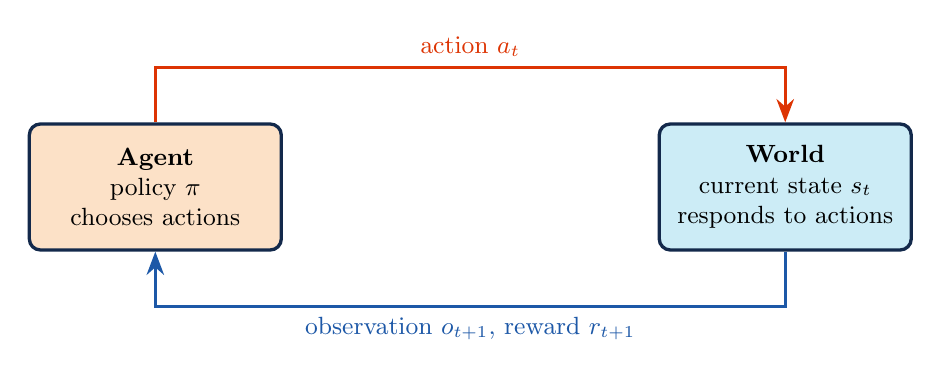
\begin{tikzpicture}[
        >=Stealth,
        box/.style={draw=ThemePrimary, very thick, rounded corners, minimum width=3.2cm,
                    minimum height=1.6cm, align=center, font=\small},
        lab/.style={font=\small}
    ]
        \node[box, fill=ThemeHighlight!25] (agent) at (0,0) {\textbf{Agent}\\ policy $\pi$ \\ chooses actions};
        \node[box, fill=ThemeSoftBlue!20] (world) at (8,0) {\textbf{World}\\ current state $s_t$\\ responds to actions};
        \draw[->, very thick, ThemeSecondary] (agent.north) -- ++(0,0.7) -| node[lab, above, pos=0.25] {action $a_t$} (world.north);
        \draw[->, very thick, ThemeAccent] (world.south) -- ++(0,-0.7) -| node[lab, below, pos=0.25] {observation $o_{t+1}$, reward $r_{t+1}$} (agent.south);
    \end{tikzpicture}

    \vspace{1em}
    \begin{itemize}
        \item Observation $o_t$ is what the agent senses about the world state $s_t$.
        \item In RL, reward $r_{t+1}$ gives feedback about the task after action $a_t$.
    \end{itemize}
    \note{
        The agent observes $o_t$ and uses policy $\pi$ to choose action $a_t$.
        The upper arrow sends that action to the world, whose state changes to $s_{t+1}$.
        The lower arrow returns observation $o_{t+1}$ and task feedback $r_{t+1}$, and the loop repeats.
        Observation tells us what is sensed; reward tells us how the task scores the interaction.
        Neither gives the complete physical state.
        For example, similar images can hide different cup velocities, so earlier observations and actions can matter.
        A POMDP describes this same loop mathematically, which is the next step.
    }
\end{frame}

\begin{frame}{The Agent--World Loop as a POMDP}
    \small
    The agent--world loop can be described as a partially observable Markov decision process (POMDP):

    \medskip
    \begin{tabularx}{\linewidth}{@{}l X@{}}
        \toprule
        States $s_t$ & The world's physical situation, including the robot's body \\
        Actions $a_t$ & Commands chosen by the agent \\
        Transition $T(s_{t+1} \mid s_t, a_t)$ & Distribution of the next state after an action \\
        Observation $O(o_t \mid s_t)$ & Distribution of what the agent senses in a state \\
        Reward $R(s_t, a_t)$ & Expected immediate task feedback \\
        \bottomrule
    \end{tabularx}

    \medskip
    The agent receives observations rather than direct access to the full state.
    The state evolves under actions; the agent senses it through observations.
    \note{
        This table gives mathematical names to the parts of the interaction loop.
        State describes the underlying situation; transition describes how an action changes it.
        Observation describes what the agent senses, and reward gives immediate task feedback.
        Partial observability means the agent receives incomplete information, such as an image without contact forces or velocity.
        History can help infer what is hidden.
        The POMDP describes the problem; the agent may still need to learn its dynamics from data.
        Here the observation function depends only on state; general formulations can also include the preceding action.
        That leads to a learned world model.
    }
\end{frame}

\begin{frame}{What a World Model is}
    \begin{block}{World model}
        Given the history of observations and actions
        \[
            H_t = (o_0, a_0, o_1, a_1, \ldots, a_{t-1}, o_t)
        \]
        and a candidate action $a_t$, a \textbf{world model} predicts a
        probability distribution over the next observation $o_{t+1}$:
        \[
            p_{\theta}\!\left(o_{t+1} \mid H_t, a_t\right)
        \]
        where $\theta$ denotes the model's learned parameters.
    \end{block}

    \begin{itemize}
        \item \textbf{Policy:} ``What should I do?''
        \item \textbf{World model:} ``What would happen if I did this?''
    \end{itemize}
    \note{
        $H_t$ contains observations through $o_t$ and the actions already taken.
        The candidate $a_t$ is separate because we are asking what would happen if we chose it now.
        The model predicts a distribution over the next observation, using parameters $\theta$ learned from interactions.
        A distribution can represent several possible outcomes.
        For the cup, pushing and doing nothing should produce different predictions.
        The policy chooses an action; the world model predicts its consequences.
        Prediction alone does not say which outcome is desirable, so next we distinguish dynamics, value, and policy.
    }
\end{frame}

\begin{frame}{What a World Model is \emph{NOT}}
    \centering
    \footnotesize
    \begin{tabularx}{\linewidth}{@{}l l l X@{}}
        \toprule
        Component & Predicts & Policy-dependent? & Belongs to \\
        \midrule
        Dynamics $p(s_{t+1} \mid s_t, a_t)$ & next state & no & \textbf{world model} \\
        Reward model $r(s_t, a_t)$ & immediate reward & no & world model (optional) \\
        Value $V^{\pi}(s) = \mathbb{E}_{\pi}[\sum_k \gamma^k r_{t+k}]$ & future return & \textbf{yes} & agent (critic) \\
        Policy $\pi(a_t \mid s_t)$ & action & -- & agent (actor) \\
        \bottomrule
    \end{tabularx}

    \note{
        Dynamics and reward describe immediate consequences of a specified state and action.
        $V^{\pi}(s)$ estimates discounted return from state $s$ when following policy $\pi$.
        Changing the policy can change the visited states and rewards, so the same state can have a different value.
        A policy that reaches the target can earn more than one that moves away, even though the environment is unchanged.
        By contrast, $T(s'\mid s,a)$ fixes both state and action, so the physical transition rule does not depend on the policy.
        A value network learns policy-associated targets; it need not receive $\pi$ explicitly.
        $V^*(s)$ instead maximises over policies.
        These are functional roles within an agent; the world model can itself be an agent component.
        We now examine V, M, and C.
    }
\end{frame}

\section{Ha \& Schmidhuber (2018)}
\subsection{Architecture Overview}
\begin{frame}{The V--M--C Architecture}
    \begin{columns}[c]
        \begin{column}{0.43\textwidth}
            \centering
            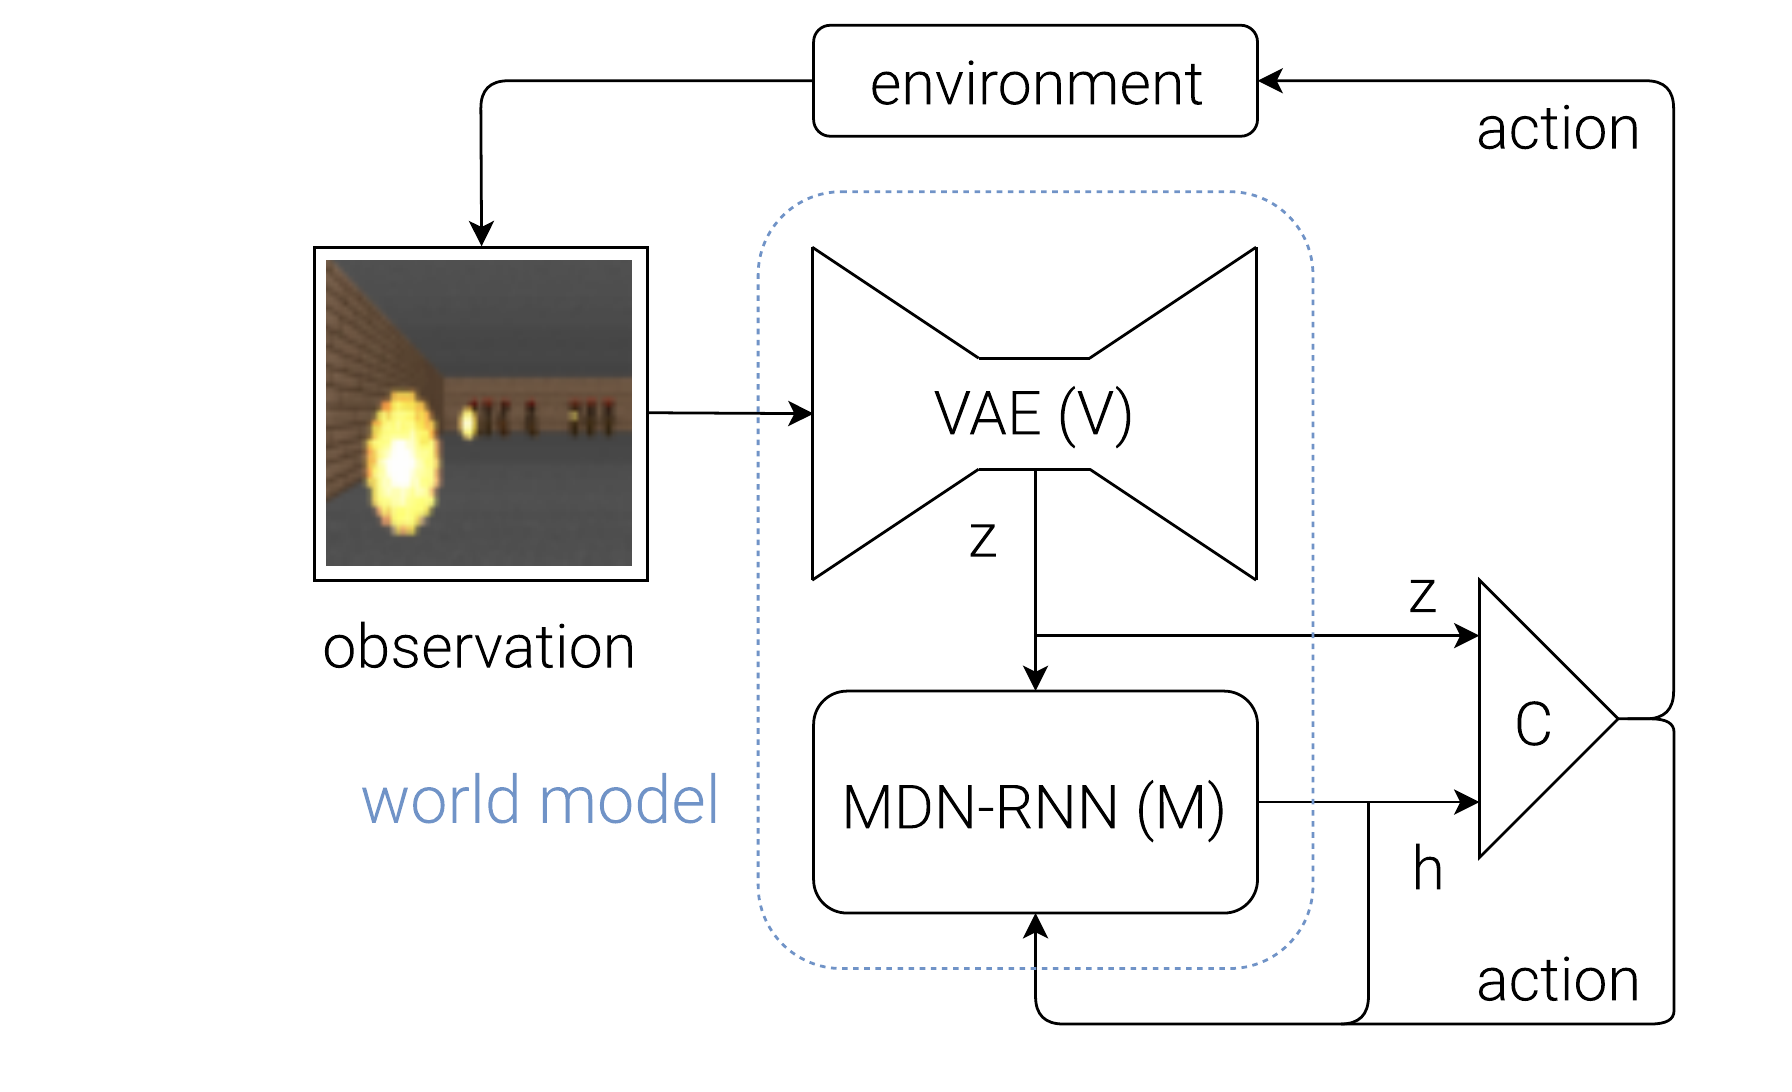
\includegraphics[width=\linewidth,height=4.7cm,keepaspectratio]{figure/ha2018-fig08-agent.png}
            \figsource{Figure 8. The V--M--C agent.}{Section 2.4.}
        \end{column}
        \begin{column}{0.53\textwidth}
            \small
            \begin{itemize}
                \item \textbf{V: vision.} Compress image $o_t$ into a latent vector $z_t$.
                \item \textbf{M: memory and prediction.} Predict the next latent vector from $z_t$, action $a_t$, and memory $h_t$.
                \item \textbf{C: controller / policy.} Choose action $a_t$ from the current latent vector and memory.
            \end{itemize}
            \medskip
            \textbf{Agent = V + M + C.}

            \smallskip
            \textbf{World model = V + M.}
            \par\smallskip
            \textit{An internal learned model of the environment.}

            \medskip
            \textbf{Design principle:} learn a large predictive representation; optimise a small controller for reward.
        \end{column}
    \end{columns}
    \note{
        In this diagram, the world is the actual game environment.
        For Car Racing, it includes the car, track, and movement rules; for VizDoom, the player, fireballs, walls, and game rules.
        The controlled car or player is part of the game state.
        The agent is the V--M--C software: it receives images and sends control commands to the game.
        V turns an image into $z_t$, a short vector of learned numbers that summarises it.
        M remembers earlier information and predicts how this latent vector changes after an action.
        C uses the current latent vector and memory to choose that action.
        Together, V, M, and C form the agent; V plus M form its internal world model.
        The world model represents the game, but is not the actual game or its full state.
        During dream training, M supplies simulated transitions to C, so model errors can affect transfer.
        We start with how V summarises an image.
    }
\end{frame}

\subsection{Vision (V)}
\begin{frame}{V: Vision with a Convolutional VAE}
    \begin{columns}[c]
        \begin{column}{0.36\textwidth}
            \centering
            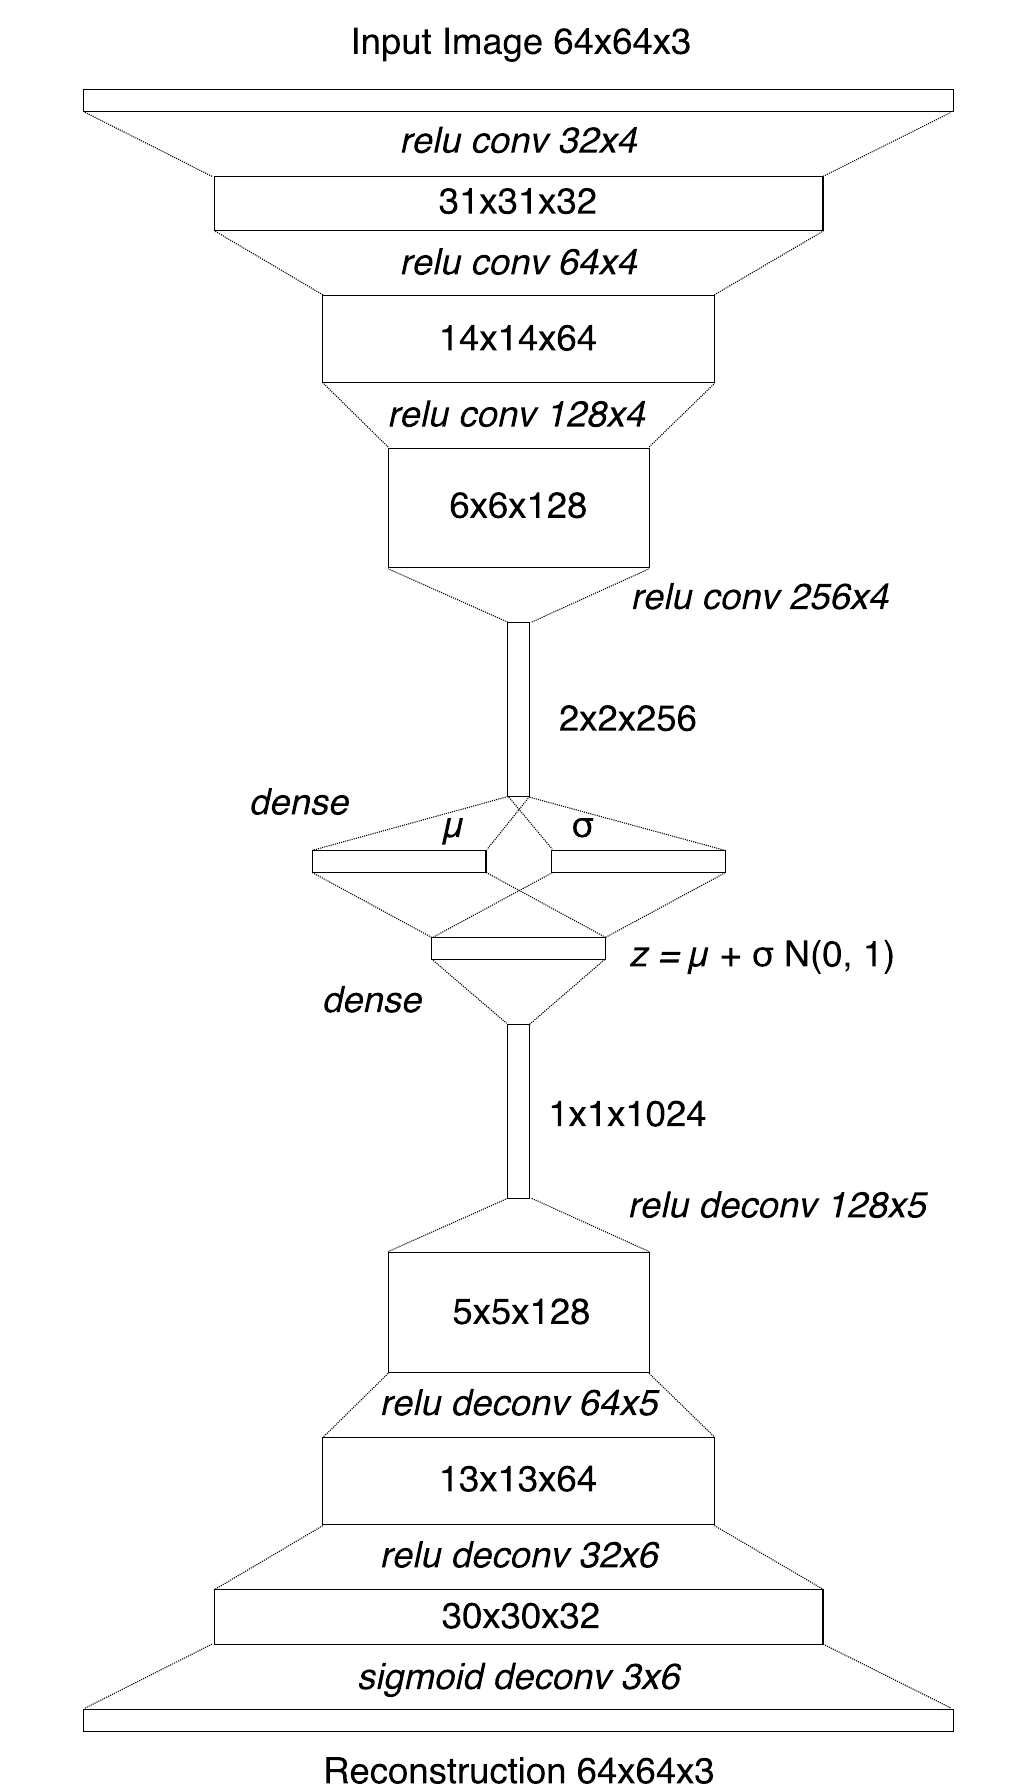
\includegraphics[width=\linewidth,height=5.35cm,keepaspectratio]{figure/ha2018-fig22-convvae.png}
            \figsource{Figure 22. The complete ConvVAE.}{Appendix A.1.}
        \end{column}
        \begin{column}{0.60\textwidth}
            \small
            \textbf{Architecture}
            \begin{itemize}
                \item Encoder: four convolutional layers compress a $64\!\times\!64$ RGB image.
                \item Sample from the encoder's Gaussian:
                    \[z_t=\mu_t+\sigma_t\odot\epsilon,\qquad \epsilon\sim\mathcal{N}(0,I).
                    \]
                \item Decoder: four transposed convolutions.
            \end{itemize}
            \textbf{Training:} reconstruction + KL; no reward.

            \medskip
            \textbf{Design choices}
            \begin{itemize}
                \item \textbf{Compact latent vector:} 32 values (Car Racing); 64 (VizDoom).
                \item \textbf{Gaussian prior:} KL encourages encoder distributions towards $\mathcal{N}(0,I)$.
            \end{itemize}
        \end{column}
    \end{columns}
    \note{
        V makes a small learned summary of the current image: the latent vector $z_t$.
        Its entries are learned features, not hand-labelled quantities such as position or speed.
        VAE means variational autoencoder: an encoder compresses the image, and a decoder learns to reconstruct it.
        Four convolutional layers learn image patterns and reduce the 64 by 64 RGB input.
        The encoder outputs a mean $\mu_t$ and spread $\sigma_t$ (standard deviation).
        The equation adds random noise scaled by $\sigma_t$ to $\mu_t$, entry by entry, to sample $z_t$.
        The decoder uses four transposed convolutions to build the image back from $z_t$.
        Reconstruction loss rewards keeping visual information.
        KL divergence measures a difference between distributions; here it encourages the encoder's distribution towards the reference Gaussian $\mathcal{N}(0,I)$.
        This regularisation is intended to make M's generated latent vectors more usable, without guaranteeing correct physics.
        The small vector makes M's prediction cheaper than using all pixels.
        V learns without task reward, and its decoder is optional when C acts.
        Next, M learns how these summaries change over time.
    }
\end{frame}

\subsection{Memory (M)}
\begin{frame}{M: Memory with an MDN--RNN}
    \begin{columns}[c]
        \begin{column}{0.46\textwidth}
            \centering
            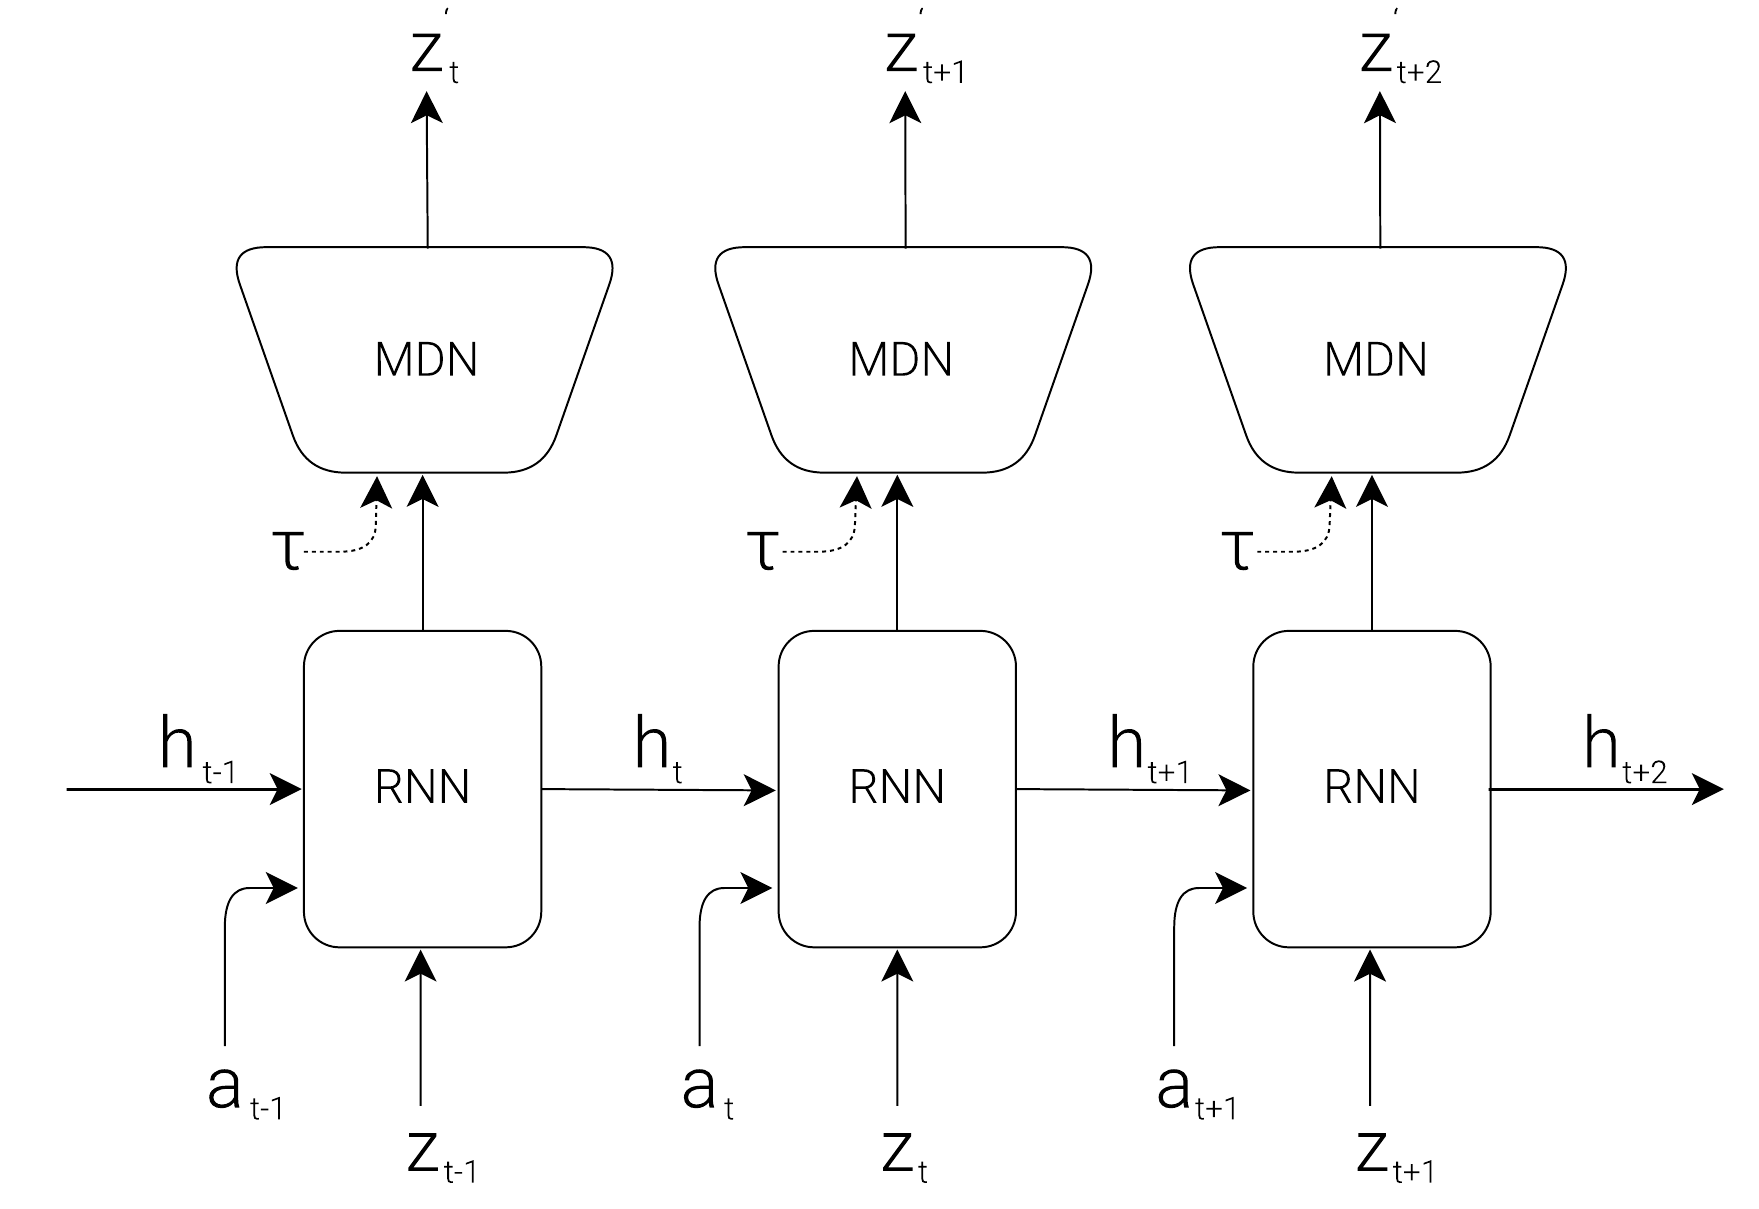
\includegraphics[width=\linewidth]{figure/ha2018-fig06-mdnrnn.png}
            \figsource{Figure 6. MDN--RNN unrolled over time.}{Section 2.2; Appendix A.2.}
        \end{column}
        \begin{column}{0.50\textwidth}
            \small
            \textbf{Architecture}
            \begin{itemize}
                \item LSTM memory: 256 units (Car Racing); 512 (VizDoom).
                \item Predict each vector entry with five Gaussian components (factored output).
                \item VizDoom: additional termination head.
            \end{itemize}
            \textbf{Training:} make recorded next latent vectors likely (negative log-likelihood).

            \medskip
            \textbf{Design choices}
            \begin{itemize}
                \item \textbf{Memory:} retain earlier information.
                \item \textbf{Uncertainty:} allow different futures.
                \item \textbf{Latent simulation:} avoid pixel rendering.
            \end{itemize}
        \end{column}
    \end{columns}
    \note{
        M predicts a distribution of possible next latent vectors from the current $z_t$, action $a_t$, and memory $h_t$.
        An LSTM, or long short-term memory network, updates memory at each step; history can reveal motion hidden in one image.
        MDN means mixture density network: it combines five Gaussian bell curves for each predicted vector entry.
        Each curve has a mean, spread, and weight; weights are nonnegative and sum to one.
        Factored means entries are predicted independently given the same inputs and memory.
        The training target is V's latent vector for the next recorded image.
        Negative log-likelihood gives lower loss when M assigns that target higher density:
        \[
        \mathcal{L}_M=-\operatorname{mean}_{t,i}\log p_{\theta,i}(z_{t+1,i}^{\mathrm{data}}\mid z_t,a_t,h_t).
        \]
        The mean averages over steps and entries; the minus sign turns likelihood maximisation into loss minimisation.
        Continuous values use density, not probability at one exact point.
        Gradients train M without task reward; VizDoom also learns when an episode ends.
        Next is C.
    }
\end{frame}

\subsection{Controller (C)}
\begin{frame}{C: A Small Controller}
    \small
    \textbf{Architecture:} join the latent vector and memory, then take weighted sums plus a bias:
    \[
        u_t=W_c[z_t;h_t]+b_c,\qquad a_t=g_{\mathrm{task}}(u_t).
    \]
    $g_{\mathrm{task}}$ applies the task's action bounds and mapping.

    \medskip
    \textbf{Training:} freeze V and M; CMA-ES optimises C using rollout return.
    \par\smallskip
    cf.CMA-ES: Covariance Matrix Adaptation Evolution Strategy.

    \medskip
    \textbf{Design choices}
    \begin{itemize}
        \item \textbf{No hidden layer:} keep reward optimisation in a small parameter space.
        \item \textbf{Read $z_t$ and $h_t$:} combine current perception with temporal predictive features.
        \item \textbf{Reward-only search:} sample controllers, rank by return, adapt the search distribution.
    \end{itemize}
    \note{
        C is the policy: it chooses an action from the current latent vector and M's memory.
        It joins those numbers, takes weighted sums, and adds a bias; this is the affine map in the equation.
        The task mapping then puts outputs into allowed ranges or discrete choices.
        In Car Racing, 32 visual values plus 256 memory values produce steering, acceleration, and braking, using 867 parameters.
        C has no hidden layer, so reward optimisation searches a small set of parameters.
        CMA-ES means Covariance Matrix Adaptation Evolution Strategy, a gradient-free way to search for good controller weights.
        It tries controllers sampled from a Gaussian distribution, runs them, and ranks their total rewards.
        Better controllers guide where to search next.
        Covariance learns which parameter changes work together; step size controls how large those changes are.
        V and M stay fixed during this search.
        The Gaussian is over controller parameters, not future observations.
        The paper tries 64 candidates per generation, scoring each over 16 seeded rollouts.
        Next we connect this search to the full training procedure.
    }
\end{frame}

\subsection{Training Procedure}
\begin{frame}{Why Train V, M, and C Separately?}
    \small
    \textbf{Start with data:} collect 10,000 random-policy rollouts for each environment.

    \medskip
    \begin{tabularx}{\linewidth}{@{}l X X@{}}
        \toprule
        Stage & Learning signal & What is learned \\
        \midrule
        1. Train V & Reconstruction + KL & Compact visual representation \\
        2. Train M & Recorded next latent vectors & Action-conditioned predictive memory \\
        3. Optimise C & Rollout return, using CMA-ES & Behaviour from fixed V/M features \\
        \bottomrule
    \end{tabularx}

    \medskip
    \textbf{Design rationale:} learn perception and dynamics from observation data;
    reserve reward optimisation for the small controller.

    \medskip
    \textbf{Two uses of the same design}
    \begin{itemize}
        \item \textbf{Car Racing:} optimise C in the actual environment using V/M features.
        \item \textbf{VizDoom:} optimise C inside M's latent simulator, then test in the actual game.
    \end{itemize}
    \note{
        Random interaction first supplies images, actions, and their consequences.
        V learns image compression, then M learns prediction from the encoded sequences.
        With V and M fixed, C is optimised for task return.
        The design gives the large networks reconstruction and prediction targets, while reward optimisation searches only the small controller.
        This is staged training, not end-to-end reward training of all three networks.
        For harder tasks, the paper discusses collecting new data as the policy reaches unfamiliar states.
        Car Racing optimises C in the actual game; VizDoom optimises it inside M's latent simulator and tests it in the actual game.
        Let us compare those two loops.
    }
\end{frame}

\begin{frame}{Actual Environment vs.\ Dream}
    \small
    \begin{tabularx}{\linewidth}{@{}l X X@{}}
        \toprule
        & Actual game & Dream: M's latent simulator \\
        \midrule
        Current latent vector $z_t$ & V encodes the current image $o_t$ & M supplies a sampled latent vector \\
        Next latent vector $z_{t+1}$ & V encodes the game's next frame & M samples the next latent vector \\
        M's role & Update predictive memory & Memory + latent transitions \\
        C's inputs & $z_t$ plus recurrent memory & $z_t$ plus recurrent memory \\
        V during control & Encoder processes each image & Encoder bypassed; decoder optional for viewing \\
        \bottomrule
    \end{tabularx}

    \medskip
    \textbf{Why bypass V?} The dream already provides latent vectors in V's latent space;
    there is no rendered frame to encode.

    \medskip
    \textbf{The latent vector is still used.} C reads the \emph{current} $z_t$ and memory;
    M's sampled $z_{t+1}$ becomes the current latent vector at the next step.

    \note{
        In the actual game, V encodes the current image, and C reads that latent vector plus M's memory to choose an action.
        The game advances, M updates memory from the latent vector and action, and V encodes the new image at the next decision.
        In the dream, M instead supplies the next latent vector from its predicted distribution.
        That sampled latent vector becomes the current observation for the next step.
        V's encoder is bypassed because there is no image to compress; its decoder is optional for human viewing.
        The latent vector is still used: $z_t$ represents the current observation, while memory carries temporal context.
        In VizDoom, memory includes both the LSTM output and cell state.
        The experiments test whether this setup supports actual-game control and transfer.
    }
\end{frame}

\subsection{Car Racing}
\begin{frame}{Car Racing: Predictive Features for Control}
    \begin{columns}[c]
        \begin{column}{0.36\textwidth}
            \centering
            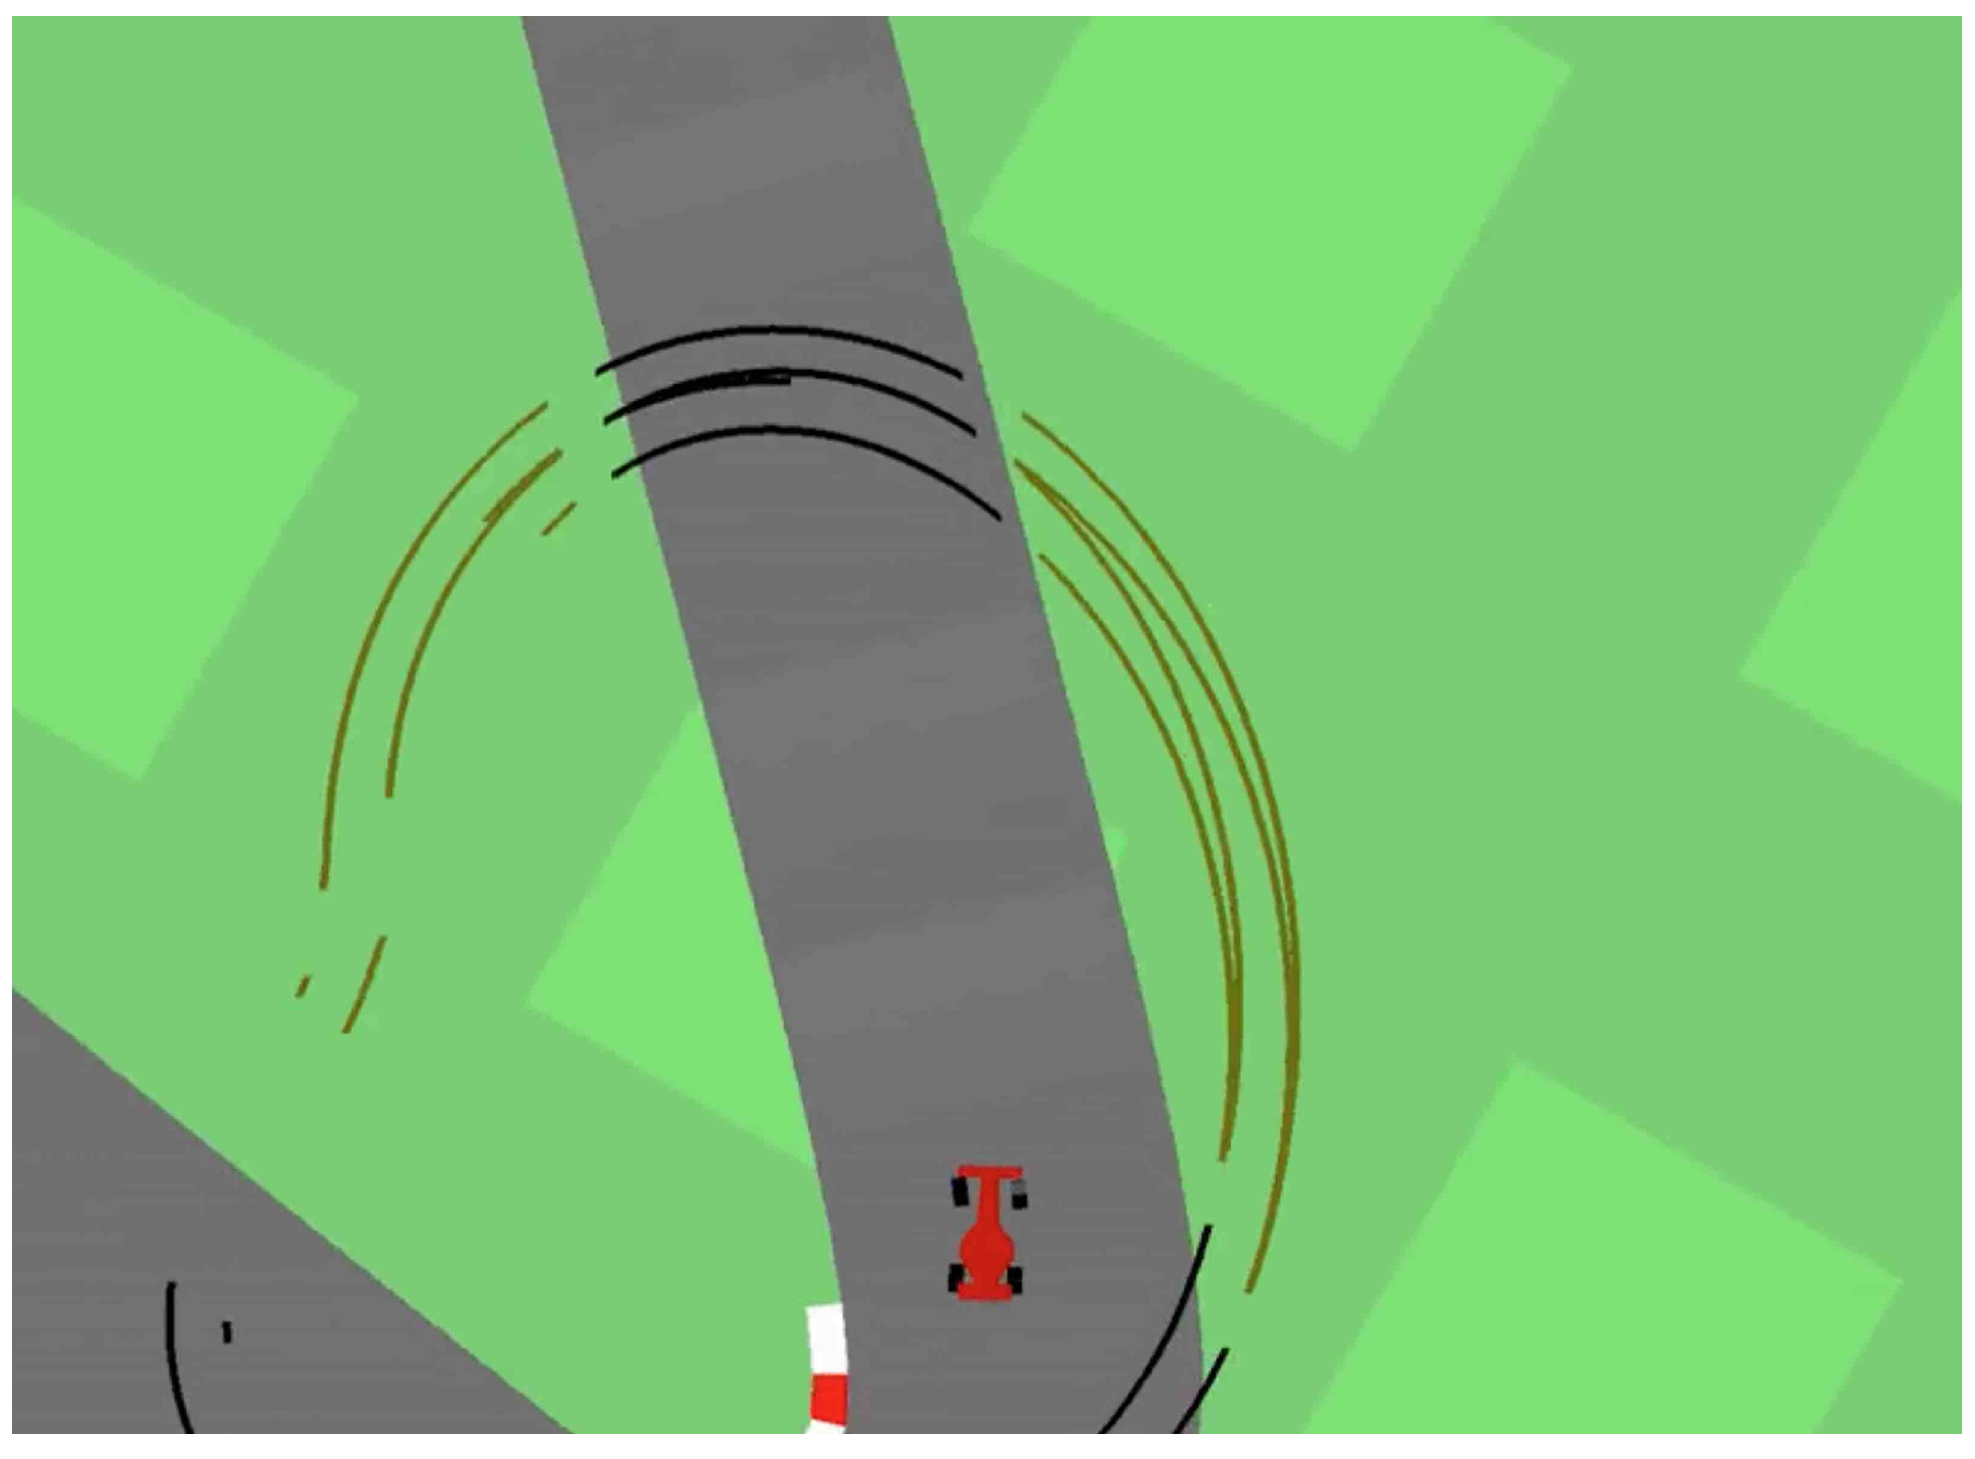
\includegraphics[width=\linewidth,height=3.2cm,keepaspectratio]{figure/ha2018-fig09-carracing.png}
            \figsource{Figure 9. CarRacing-v0.}{Section 3; Table 1.}
            \medskip
            \small
            \begin{tabular}{lr}
                \toprule
                Features & Score \\
                \midrule
                V only & $632\pm251$ \\
                \textbf{V + M} & $\mathbf{906\pm21}$ \\
                \bottomrule
            \end{tabular}
            \par\smallskip
            {\footnotesize 100 random tracks; solve: $\geq900$.}
        \end{column}
        \begin{column}{0.60\textwidth}
            \small
            \textbf{Task:} navigate randomly generated tracks from images.
            Reward favours visiting track tiles while penalising elapsed time.
            \par\medskip
            \textbf{Actions:} steering, acceleration, braking.
            \par\medskip
            \textbf{Design}
            \begin{itemize}
                \item V: 32-dimensional latent vector; M: 256-unit LSTM.
                \item C maps $[z_t;h_t]$ to three bounded controls.
                \item Learn V/M from 10,000 random rollouts; then freeze them.
                \item CMA-ES optimises C in the \textbf{actual game}.
            \end{itemize}
            \textbf{Role of M:} predictive features for C, without an explicit planning search at each decision.
        \end{column}
    \end{columns}
    \note{
        The car follows a randomly generated track from images, using steering, acceleration, and braking.
        Return rewards track coverage and penalises time.
        Random rollouts train V and M; with them fixed, CMA-ES optimises C in the actual game.
        C uses M's recurrent features without searching over imagined action sequences at each decision.
        The reported score rises from 632 with V alone to 906 with V plus M, above the solving threshold over 100 tracks.
        This shows useful recurrent features, but does not fully separate the effects of memory and predictive training.
        VizDoom next uses M as C's training environment.
    }
\end{frame}

\subsection{VizDoom}
\begin{frame}{VizDoom: Learning Inside the Dream}
    \begin{columns}[c]
        \begin{column}{0.36\textwidth}
            \centering
            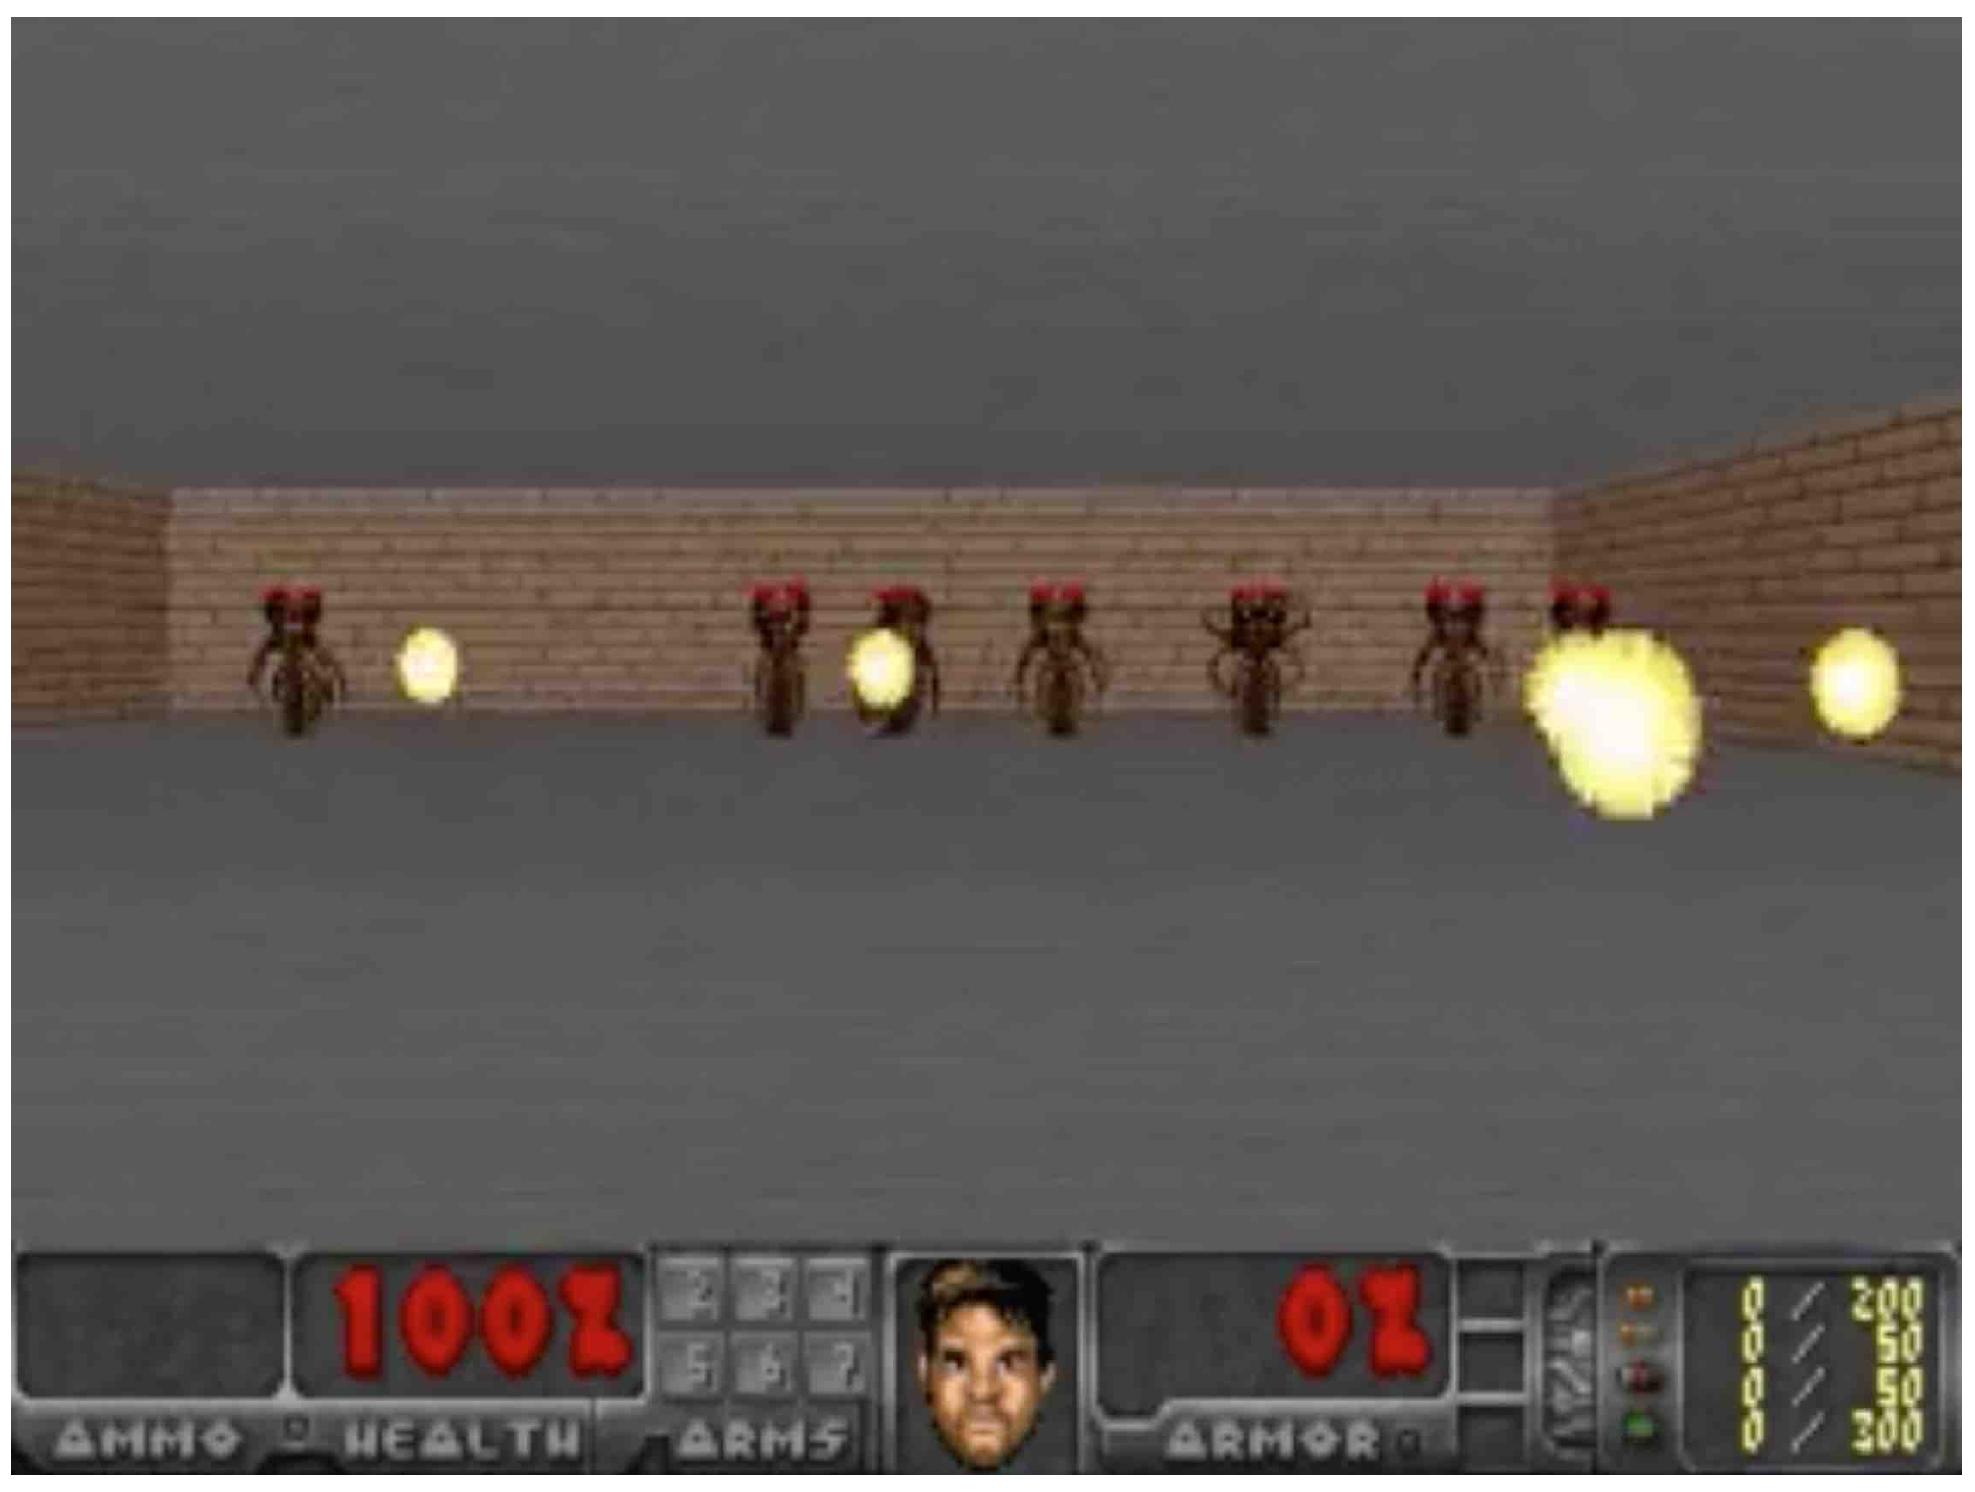
\includegraphics[width=\linewidth,height=3.2cm,keepaspectratio]{figure/ha2018-fig14-vizdoom.png}
            \figsource{Figure 14. VizDoom: Take Cover.}{Section 4; Table 2.}
            \medskip
            \small
            \setlength{\tabcolsep}{3pt}
            \begin{tabular}{lrr}
                \toprule
                $\tau$ & Dream & Actual \\
                \midrule
                0.10 & $2086\pm140$ & $193\pm58$ \\
                1.15 & $918\pm546$ & $\mathbf{1092\pm556}$ \\
                \bottomrule
            \end{tabular}
            \par\smallskip
            {\footnotesize Survival steps; actual test: 100 trials. Solve: $>750$.}
        \end{column}
        \begin{column}{0.60\textwidth}
            \small
            \textbf{Task:} dodge monsters' fireballs and stay alive.
            \par\medskip
            \textbf{Actions:} move left, stay, or move right.
            \par\medskip
            \textbf{Design}
            \begin{itemize}
                \item V: 64-dimensional latent vector; M: 512-unit LSTM plus a termination head.
                \item C uses $[z_t;h_t;c_t]$; a scalar output maps to three choices.
                \item Learn V/M from 10,000 recorded random rollouts in the actual game.
                \item CMA-ES optimises C \textbf{only inside M's latent simulator}, then tests it in the actual game.
            \end{itemize}
            \textbf{Design check:} sampling temperature affects model exploitation and transfer.
        \end{column}
    \end{columns}
    \note{
        Take Cover requires moving sideways to avoid fireballs; return is survival time, up to 2100 steps.
        Random play in the actual game trains V and M.
        M predicts both the next latent vector and termination, allowing a complete latent simulator.
        C reads the current latent vector and both LSTM memory vectors.
        CMA-ES trains C entirely in the dream, then tests the policy in the actual game.
        Low temperature gives excellent dream survival but poor transfer; the higher setting reaches a reported actual-game mean of 1092 steps.
        Added randomness made exploitation harder in this setup, without guaranteeing an accurate model.
        These results expose both the benefit and risk of learned simulation.
    }
\end{frame}

\subsection{Lessons and Limitations}
\begin{frame}{Architectural Lessons and Limitations}
    \begin{itemize}
        \item \textbf{Capacity allocation:} a large V/M representation supports a small reward-optimised controller.
        \item \textbf{V's bottleneck:} reconstruction retains visual information, which may differ from what control needs.
        \item \textbf{M's memory:} a finite LSTM state summarises history; simulated futures advance one step at a time.
        \item \textbf{Simulation errors:} C can exploit M; more stochastic dreams helped transfer but did not eliminate model bias.
    \end{itemize}
    \note{
        V and M learn useful representations before reward optimisation trains the small C.
        However, V's reconstruction objective can preserve visual detail that differs from what control needs.
        M compresses history into finite memory and simulates one step at a time.
        Its errors can affect both the features C reads and the simulated experience used to train C.
        The temperature results show why a high dream score alone does not establish reliable transfer.
        The main design separates perception, prediction, and control; the key check is whether their interfaces preserve task-relevant information.
        Let us summarise those choices.
    }
\end{frame}

% =============================================================================
\section{Conclusion}
% =============================================================================

\begin{frame}{Summary}
    \begin{itemize}
        \item \textbf{V:} a convolutional VAE compresses each image into $z_t$.
        \item \textbf{M:} an LSTM with a mixture-density head predicts $z_{t+1}$ from $z_t$, $a_t$, and memory.
        \item \textbf{C:} a small controller reads the current latent vector and recurrent features to choose actions.
        \item \textbf{Training:} learn V and M from recorded interactions, then optimise C for rollout return.
        \item \textbf{Evidence:} predictive features help Car Racing; latent-simulator training transfers in VizDoom, with sensitivity to model errors.
    \end{itemize}
    \note{
        V compresses images, M predicts latent changes, and C chooses bounded actions from vision and memory.
        Most representation learning uses recorded observations, while reward optimisation trains the small controller.
        Car Racing shows predictive features supporting control in the actual game.
        VizDoom shows dream-trained behaviour transferring to the game, with sensitivity to model errors.
        We now compare this separation of prediction and control with recent models that use latent planning or joint future-and-action generation.
    }
\end{frame}

\begin{frame}{Comparison with Recent Models}
    \small
    \begin{tabularx}{\linewidth}{@{}>{\raggedright\arraybackslash}p{2.7cm} >{\raggedright\arraybackslash}X >{\raggedright\arraybackslash}X >{\raggedright\arraybackslash}X@{}}
        \toprule
        Model & Prediction & Action selection & Main design difference \\
        \midrule
        \href{https://arxiv.org/abs/1803.10122}{\textbf{World Models}} (2018) & VAE latent vectors via MDN--LSTM & Small C, optimised by CMA-ES & Separate V/M/C; task-specific game data \\
        \addlinespace[0.25em]
        \href{https://arxiv.org/abs/2506.09985}{\textbf{V-JEPA 2-AC}} (2025) & Future JEPA features & MPC towards an image goal & Web-video pretraining, then robot dynamics \\
        \addlinespace[0.25em]
        \href{https://arxiv.org/abs/2602.15922}{\textbf{DreamZero}} (2026) & Future video and action chunks & Joint video--action diffusion policy & Future generation coupled to executable actions \\
        \addlinespace[0.25em]
        \href{https://arxiv.org/abs/2603.17240}{\textbf{GigaWorld-Policy}} (2026) & Actions + future video during training & Action output can skip video generation & Causal masking makes future video optional at inference \\
        \bottomrule
    \end{tabularx}
    \par\medskip
    \textbf{Connection:} 2018 separates prediction from control; recent designs
    use prediction for latent planning or integrate it with action generation.
    \note{
        Compare what each model predicts and how it chooses actions.
        The 2018 design learns task-specific V/M features and a separate reward-optimised C.
        V-JEPA 2-AC starts from video pretraining, adds action-conditioned robot dynamics, and plans towards an image goal.
        The AC variant takes robot actions; base V-JEPA 2 pretraining does not.
        DreamZero jointly predicts future video and executable action chunks in one diffusion policy.
        GigaWorld-Policy trains with action and future-video targets, but its causal mask lets deployment skip video generation.
        All use future-related information; representation, data scale, and the connection to action selection differ.
        This is an architectural comparison, not a comparison of game scores with robot success rates.
    }
\end{frame}

\begin{frame}
    \centering
    {\Huge Thank you!}

    \note{
        Thank you.
        We can return to the architecture, a component's design choices, or the difference between the two training environments.
        The references are next if we want to check a result.
    }
\end{frame}

\begin{frame}{References}
    \tiny
    \begin{itemize}
        \item K.~Craik. \emph{The Nature of Explanation}. Cambridge University Press, 1943.
        \item L.~P.~Kaelbling, M.~L.~Littman, and A.~R.~Cassandra. Planning and acting in partially observable stochastic domains. \emph{Artificial Intelligence}, 1998.
        \item R.~S.~Sutton. Integrated architectures for learning, planning, and reacting (Dyna). \emph{ICML}, 1990.
        \item R.~S.~Sutton and A.~G.~Barto. \emph{Reinforcement Learning: An Introduction}, 2nd ed. MIT Press, 2018.
        \item D.~Ha and J.~Schmidhuber. World Models. \emph{arXiv:1803.10122}, 2018.
        \item M.~Assran et al. V-JEPA 2: Self-supervised video models enable understanding, prediction and planning. \emph{arXiv:2506.09985}, 2025.
        \item N.~Hansen. The CMA Evolution Strategy: A Tutorial. \emph{arXiv:1604.00772}, 2016.
        \item D.~Hafner et al. Learning latent dynamics for planning from pixels (PlaNet), \emph{ICML} 2019; Dream to control (Dreamer), \emph{ICLR} 2020.
        \item J.~Schrittwieser et al. Mastering Atari, Go, chess and shogi by planning with a learned model (MuZero). \emph{Nature}, 2020.
        \item Y.~LeCun. A path towards autonomous machine intelligence. \emph{OpenReview}, 2022.
        \item J.~Bruce et al. Genie: Generative interactive environments. \emph{ICML}, 2024.
        \item A.~Brohan et al. RT-2: Vision-language-action models. 2023. \quad M.~J.~Kim et al. OpenVLA. 2024. \quad K.~Black et al. $\pi_0$. 2024.
        \item Y.~Du et al. Learning universal policies via text-guided video generation (UniPi). \emph{NeurIPS}, 2023.
        \item Motus: A unified latent action world model. \emph{arXiv:2512.13030}, 2025.
        \item S.~Ye et al. World action models are zero-shot policies (DreamZero). \emph{arXiv:2602.15922}, 2026.
        \item GigaAI. GigaWorld-Policy: An efficient action-centered world--action model. \emph{arXiv:2603.17240}, 2026.
        \item X.~Zhang, X.~Zeng, and W.~Zhang. From world models to world action models: A concise tutorial for robotics. \emph{arXiv:2607.00836}, 2026.
        \item Z.~Lu et al. World-action models for robot learning and control: A survey. \emph{arXiv:2609.16074}, 2026.
    \end{itemize}
    \note{
        The original paper and appendix provide the figures, architecture details, and experiment results.
        The other references support the definitions and recent-model comparison.
    }
\end{frame}

\end{document}
